\section{Orden de archivos}
Este es el arbol de directorios final

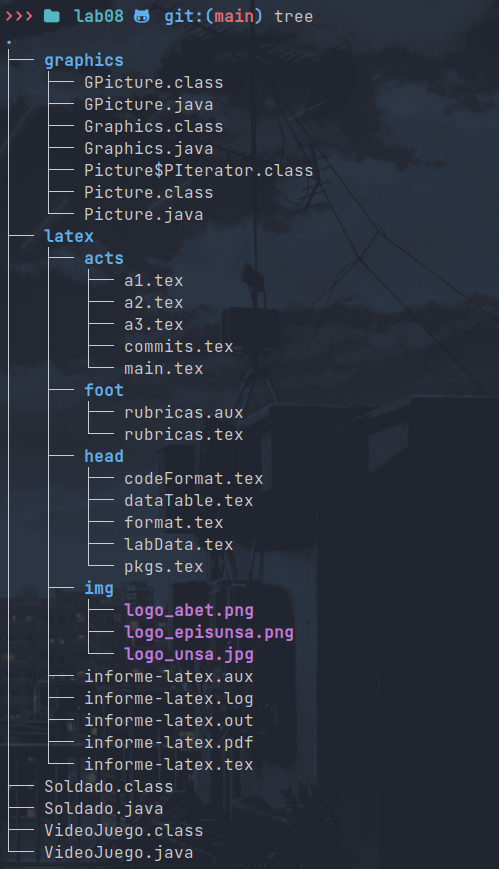
\includegraphics [width=0.26\textwidth] {img/tree.jpg}


\section{Actividades iniciales: Crea un proyecto llamado Laboratorio 7}
Se creo el directorio lab07, y se copio a el los archivos de los anteriores laboratorios para reciclar partes de codigo

\begin{itemize}
  \item Se importaron las clases Soldado y Videojuego
  \item El soldado tiene las especificaciones requeridas como atributos
  \begin{itemize}
    \item Nombre
    \item Puntos de vida
    \item Fila
    \item Columna
  \end{itemize}
  \item Para el tablero, se sigue utilizando la biblioteca graphics, la unica indicacion es que se use la estructura de datos mas adecuada, lo que me sugiere que es a libre eleccion, por lo tanto se uso un array bidimensional simple para el tablero

  \subsection{Regresando el modelo de ArrayList a array simple}
  \begin{itemize}
    \item Como dije anteriormente, importamos las anterioes clases de videojuego, y en la clase que importamos, el tablero esta representado con un ArrayList
    \item Para trabajar mejor se hizo el pase de ArrayList a array simple
    \item Se logro eso, cambiando los lugares donde trabaja ArrayList
  \end{itemize}

\end{itemize}
